% !TeX root = ./main.tex
\documentclass[main]{subfiles}
\begin{document}
\chapter{Компактность}
\section{Компактность}
\begin{definition}
    $(X, \Omega)$ -- топологическое пространство,
    \[\{U_i\}_{i \in I} \subset \Omega: \bigcup_i U_i = X.\]
    Такое $\{U_i\}_{i \in I}$ -- покрытие $X$. (точнее открытое покрытие)

    $\{V_j\}_{j \in J}$ называется подпокрытием $\{U_i\}_{i \in I}$, если
    $\forall j\ \exists i: V_j = U_i$ и $\{V_j\}$ -- покрытие.
\end{definition}

По умолчанию: покрытие = открытое покрытие.

\begin{definition}
    $X$ называется компактным, если $\forall \{U_i\}_{i \in I}$ -- покрытия $X$
    можно выбрать $U_{i_1}, ..., U_{i_n}$ конечное подпокрытие.
\end{definition}

В старых учебниках это называется бикомпактностью.

\begin{definition}
    $A \subset X$ компактно, если $A$ компактно в индуцированной топологии
    или $\forall \{U_i\}_{i \in I} \subset \Omega: \bigcup U_i \supset A \ \exists U_{i_1}, ..., U_{i_n}:
        \bigcup_{k=1}^n U_{i_k} \supset A$
\end{definition}

\begin{example}
    $X$ -- антидискретное пространство, значит $X$ компактно.
\end{example}

\begin{example}
    $X$ -- конечное, тогда $X$ компактно

    $X = \{x_1, ..., x_n\}$ и $\{U_i\}_{i \in I}$ -- некоторое покрытие.
    Различных $U_i$ не более $2^n$, поэтому считаем весь набор $U_i$ конечным.
\end{example}

\begin{example}
    Бесконечное дискретное пространство не компактно.

    $X = \bigcup_{x_i \in X} \{x_i\}$, $\{x_i\}$ -- открыто.
    Ни одно из подмножеств нельзя выкинуть. Конечного подпокрытия быть не может.
\end{example}

\begin{example}
    Топология Зариского компактна.

    Пусть $X = \bigcup_{i \in I} U_i$, $U_{i_0} = X \setminus \{x_1, x_2, ..., x_n\}$.
    Но $x_1 \in U_{i_1}, x_2 \in U_{i_2},..., x_n \in U_{i_n}$.
    $\{U_{i_k}\}_{k=0}^n$ -- покрытие $X$.
    Из этого следует, что $\forall A \subset X$ компактно.
\end{example}

\begin{example}
    Стрелка: топология на $\R$, где $(x; +\infty) + \varnothing + \R$ открытые.
    Сама по себе не компактна.

    $U_i = (-i; +\infty), \bigcup_{i=1}^\infty U_i = \R$.
    Но конечного набора, который бы давал $\R$ не существует.

    Какие подмножества стрелки является компактными?

    $A = [0, \infty)$, такое $A$ компактно.

    $B \subset \R$, $B$ компактно тогда и только тогда, когда $\inf B \in B$.
    Если $\inf B = x_0$ и $x_0 \not\in B$, тогда $U_n = (x_0 + 1/n; +\infty)$.
    Тогда $\bigcup_{n=1}^\infty U_n \supset B$, но конечное подпокрытие выбрать нельзя.
\end{example}

\begin{example}
    $\R^{(n)}$ со стандартной топологией. Само по себе не компактно (см. стрелку): $U_i = (-i; +\infty)$

    Какие подмножества $\R^n$ компактны? Читайте далее!
\end{example}

\begin{theorem}\label{compact:1}
    $X$ -- компактное пространство. $A$ -- замкнутое подмножество в $X$, тогда $A$ компактно.
\end{theorem}
\begin{proof}
    Пусть $\{U_i\}_{i \in I}$ покрывает $A$. $\{U_i\}\ \cup\ \{X \setminus A\}$ -- открытое покрытие $X$,
    значит существует конечное подпокрытие. Уберем из него $X \setminus A$ (если есть), получим конечное подпокрытие $A$.
\end{proof}

\begin{theorem}\label{compact:2}
    $f: X \to Y$ непрерывно. $A \subset X$. $A$ компактно, тогда $f(A)$ компактен.
\end{theorem}

\begin{proof}
    Пусть $\{U_i\}_{i \in I}$ покрывают $f(A)$. Тогда $\{f^{-1} (U_i)\}$ открытое покрытие $A$.
    Тогда \[\exists U_{i_1}, ..., U_{i_n}: \bigcup_{k =1 }^n f^{-1}(U_{i_k}) \supset A,\]
    значит $U_{i_1}, ..., U_{i_n}$ покрывают $f(A)$
\end{proof}
\begin{corollary}
    Компактность -- топологическое свойство.
\end{corollary}

\begin{theorem}[Тихонова]
    $\prod_{i \in I} X_i$ компактно $\Leftrightarrow \forall i\ X_i$ компактно.
\end{theorem}
\begin{proof}
    Не будет.
\end{proof}

\begin{theorem}\label{compact:3}
    $X$ и $Y$ компактны $\Leftrightarrow X \times Y$ компактно
\end{theorem}
\begin{proof}
    В обратную сторону: $p: X\times Y \to X$ -- проекция, она непрерывна.
    $X\times Y$ компактно, значит по теореме \ref{compact:2} $p(X \times Y) = X$ тоже компактно.

    Прямо. рассмотрим любое открытое покрытие $X \times Y$:
    \begin{enumerate}
        \begin{minipage}{0.45\textwidth}
            \item Считаем, что это покрытие прямоугольными множествами, т.е. $\{U_i \times V_i\}_{i \in I}$,
            $U_i$ открыто в $X$, $V_i$ открыто в $Y$.
            Достаточно выбрать конечное подмножество из него.
        \end{minipage}
        \begin{minipage}{0.45\textwidth}
            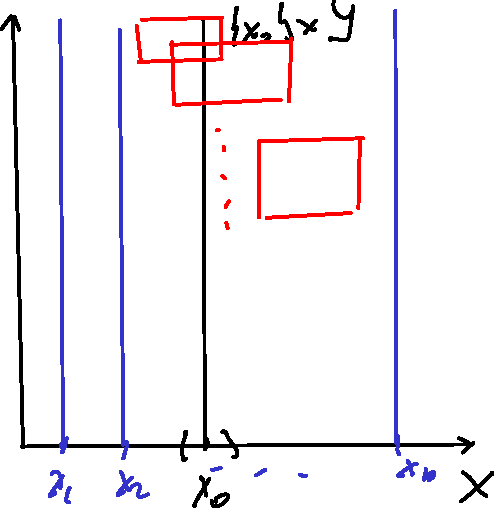
\includegraphics[width=\textwidth]{coverage.pdf}
        \end{minipage}
        \item $\forall x_0 \in X,\ \{x_0\}\times Y \simeq Y$ в $X\times Y$.
              Существует минимальное покрытие $U_1 \times V_1, ..., U_n \times V_n$, которое покрывает $\{x_0\} \times Y$,
              значить $V_1, ..., V_n$ покрывает $Y$.

              $W_{x_0} \coloneqq \bigcap_{i=1}^n U_i$ -- открытое в $X$ подмножество.
              $x_0 \in W_{x_0}$, тогда $\{W_{x_0}\}_{x_0 \in X}$ -- покрытие $X$, следовательно существует $W_{x_1}, ..., W_{x_k}$ -- конечное подпокрытие.
              \[W_{x_j} \leftrightarrow \{U_{j_1} \times V_{j_1}, ..., U_{j_{n_j}} \times V_{j_{n_j}}\}\]
              Возьмем все множества, соответствующие $W_j$. Это конечный набор. Почему покрытие?
              $\forall (x,y) \in X \times Y,\ x\in W_{x_l},\ (x_l, y) \in U_i \in V_i$
              ($U_i \times V_i$ из нашего набора). $x \in U_i$ и $y \in V_i$, $(x,y) \in U_i \times V_i$
    \end{enumerate}
\end{proof}

\section{Компактность и хаусдорфовость}
\begin{axiom}[Хаусдорфа]
    $X$ называется хаусдорфовым, если $\forall x_0 \neq x_1 \in X\ \exists U_{x_0}, U_{x_1} : U_{x_0} \cap U_{x_1} = \varnothing$
\end{axiom}
\begin{example}
    Любое метрическое пространство хаусдорфово.
    \begin{gather*}
        U_{x_0} = B(x_0, \rho(x_0, x_1) /2)\\
        U_{x_1} = B(x_1, \rho(x_0, x_1) /2)
    \end{gather*}
\end{example}
\begin{remark}
    X хаусдорфово, $A \subset X \implies A$ хаусдорфово.
\end{remark}

\begin{theorem}\label{compact:4}
    $X$ -- хаусдорфово пространство. $A \subset X$, $A$ компактно в $X$, тогда $A$ замкнуто.
\end{theorem}
\begin{remark}
    Докажем, что $X \setminus A$ открыто.
    Для этого возьмем любой $x_0 \in X \setminus A$. Найдем $U_{x_0} \cap A = \varnothing$
    \[\bigcup_{x_0} = X \setminus A \text{ - открыто}\]
    Это базовая схема как доказать замкнутость подмножеств.
\end{remark}
\begin{proof}
    Рассмотрим $\forall y \in A \ \exists U_{x_0 y}$ и $V_y$ -- окрестности:
    $x_0 \in U_{x_0y}, y \in V_y, \ U_{x_0y} \cap V_y = \varnothing$ (по хаусдорфовости).

    $\{V_y\}_{y \in A}$ -- покрывают $A$, тогда $\exists y_1, ..., y_n: V_{y_1}, ..., V_{y_n}$ -- покрытие $A$,
    рассмотрим $\bigcap_{i=1}^n U_{x_0 y_i}$ открытое подмножество, не пересекающееся с $V_{y_i} \forall i = 1, ..., n$,
    значит $\bigcap_{i = 1}^n U_{x_0y_i}$ не пересекается с $A$.
\end{proof}

\begin{corollary}
    $X$ -- компактно и хаусдорфово, $A \subset X$, тогда $A$ компактно $\Leftrightarrow A$ замкнуто.
\end{corollary}

\begin{theorem}\label{compact:5}
    $f: X \to Y$ непрерывно. $X$ компактно, $Y$ хаусдорфово. $A \subset X$, $A$ замкнутое, значит $f(A)$ замкнут.
\end{theorem}
\begin{proof}
    $A$  замкнуто, тогда по теореме \ref{compact:1}  $A$ компактно, значит по теореме \ref{compact:2}
    $f(A)$ компактен, тогда по теореме \ref{compact:4} $f(A)$ замкнут.
\end{proof}
\begin{corollary}
    $f: X \to Y$ непрерывное и биекция. $X$ компактно. $Y$ хаусдорфово.  $A$ открытое, тогда $f(A)$ открыт.
\end{corollary}
\begin{proof}
    $A$ открытое, значит $X \setminus A$ замкнутое, значит $f(X \setminus A)$ замкнут, значит $f(A)$ открыт.
    \[f(X \setminus A) = Y \setminus f(A),\text{ если $f$ биективно}\]
\end{proof}
\begin{corollary}
    $f: X \to Y$ непрерывная биекция, $X$ компактно, $Y$ хаусдорфово, тогда $f$ гомеоморфизм.
\end{corollary}

\begin{minipage}{0.45\textwidth}
    Кривые Пеано: $f: [0,1] \to [0,1] \times [0,1]$ -- непрерывное и сюръективное отображение.

    В пределе непрерывная кривая, которая заметает весь квадрат.
    Кривая Пеано не может быть биективной!
\end{minipage}
\begin{minipage}{0.45\textwidth}
    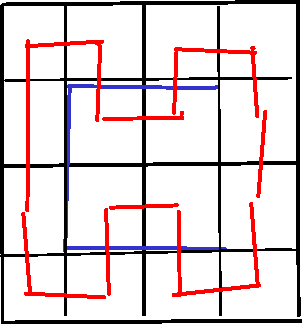
\includegraphics[width=\textwidth]{peano_curve_compact.pdf}
\end{minipage}

\section{Компактность в \texorpdfstring{$\R^n$}{R\textasciicircum n}}

\begin{lemma}[Лебега]\label{compact:6}
    $I = [0,1], \{U_i\}$ -- открытое покрытие $I$, тогда существует $\epsilon >0$
    (число Лебега, зависит от покрытия)$: \forall x_0  \in I\ (x_0 - \epsilon; x_0 + \epsilon) \subset U_i$ для некоторого $i$.
\end{lemma}
\begin{proof}
    Допустим такого $\epsilon$ не существует. $\epsilon_i \coloneqq 1/2^i$ (или  $\epsilon_i \to 0$).

    $\exists x_i: (x_i - \epsilon_i; x_i + \epsilon)$ не попадает ни в одно $U_i$.
    $\{x_i\}_{i=1}^{\infty}$ -- последовательность точек $I$.
    $\exists x_{i_j} \to x_0$ в $[0,1]$.
    $x_0 \in U_i$, $U_i$ открыто, значит $\exists \epsilon >0 : (x_0 - \epsilon; x_0 + \epsilon) \subset U_i$

    $\exists N_1:$ если $j > N_1$, то $|x_0 - x_j| < \epsilon/2$.
    Так же $\exists N_2: \epsilon_{N_2} < \epsilon/2$.
    Выберем $N\coloneqq \max\{N_1, N_2\}$, тогда
    \[(x_{i_j} - \epsilon_{i_j}; x_{i_j} + \epsilon_{i_j}) \subset (x_0 - \epsilon; x_0 + \epsilon) \subset U_i\]
    Противоречие, значит число Лебега существует.
\end{proof}

\begin{theorem}\label{compact:7}
    $[0,1]$ компактен
\end{theorem}
\begin{proof}
    $\{U_i\}$ покрывает $I = [0,1]$, тогда по теореме \ref{compact:6} $\exists \epsilon$ -- число Лебега.
    $x_0 = 0, x_k = k\epsilon \implies \exists N: x_N > 1$.
    Тогда $(x_{k-1}; x_{k+1}) = (x_k - \epsilon; x_k + \epsilon) \subset U_{i_k}$.
    Рассмотрим $U_{i_1}, U_{i_2}, ..., U_{i_{N-1}}$ -- покрытие $[0;1]$.
\end{proof}

\begin{remark}
    $(0,1)$ не компактно. $U_k = (1/k, 1)$. Нельзя выбрать конечное подпокрытие
\end{remark}
\begin{corollary}\label{compact:7:1}
    $[a_1, b_1] \times ... \times [a_n, b_n]$ компактно в $\R^n$
\end{corollary}

\begin{definition}
    $A \subset \R^n$, $A$ называется ограниченным, если $A \subset B(0, N)$, такое $N$ существует.
    Или $A \subset [a_1, b_1] \times ... \times [a_n, b_n]$
\end{definition}

\begin{theorem}[Компактность подмножества в $\R^n$]
    $A \subset \R^n$, $A$ компактно $\Leftrightarrow A$ -- замкнуто и ограниченно.
\end{theorem}
\begin{proof}
    Прямое доказательство $A$ замкнуто по \ref{compact:4}, $A$ ограниченно, иначе  $\{B(0, n)\}_{n=1}^\infty$ -- покрытие,
    из которого нельзя выбрать конечное.

    Обратное доказательство: $A$ ограниченно, значить $A \subset X = [a_1, b_1] \times ... \times [a_n, b_n]$,
    $X$ компактно по \ref{compact:7:1}, $A$ замкнуто в $X$, значит по \ref{compact:1} $A$ компактно.
\end{proof}

\begin{theorem}\label{compact:8}
    $f: X \to \R$ -- непрерывная функция, $X$ компактен, тогда $\exists x_0: f(x_0) \ge f(x)\ \forall x \in X$.
    (т.е. непрерывная функция на компакте достигает своего максимума)
\end{theorem}
\begin{proof}
    $f(X)$ компактна в $\R$, значит $f(X)$ замкнута и ограничена. Ограничена, значит $\sup f(X) < + \infty$.
    Замкнута, значит $\sup f(X) \in f(X) \implies \sup$ достигается.
\end{proof}

\begin{example}
    В прошлом семестре: брали квадратичную форму
    \[F(x,y,z) = a_{11} x^2 + a_{22}y^2 + a_{33} z^2 + 2 a_{12} xy + 2 a_{13} xz + 2 a_{23}yz\]
    Поворотом можно избавиться от двойных слагаемых.

    Для этого мы проецировали на сферу
    \[F(x,y,z)\rvert_{S^2} \qquad S^2 \coloneqq \{(x,y,z): x^2+y^2+z^2 = 1\}\]
    $(x_*, y_*, z_*)$ -- максимум $F$ на $S^2$

    $F$ -- непрерывна, $S^2$ -- компактна, значит существует максимум.
\end{example}

\begin{example}[Задача Фаньяно]
    $ABC$ -- остроугольный треугольник.
    Хотим выбрать $A' \in [BC], B' \in [AC], C' \in [AB]$,
    так чтобы $P_{A'B'C'} \to \min$.
    Ответ: это основания высот.
    \begin{center}
        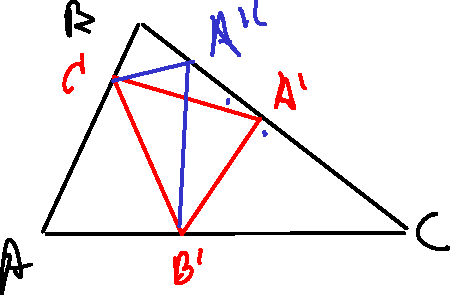
\includegraphics[width=0.5\linewidth]{fagnanos_problem.pdf}
    \end{center}
    Если $A'B'C'$ -- искомый, тогда $\angle C'A'B = \angle B'A'C$.
    Если нет, то $A'': \angle C'A''B = \angle B'A''C.$
    \[C'A'' + A''B' < C'A' + A'B'\]
    (это доказано в оптическом свойстве эллипса.)

    Значит оптимальная конфигурация: с равными соответствующими углами.
    Такое бывает, если $A',B',C'$ -- основания высот. (почему? -- упражнение)
\end{example}

\textbf{Принцип.} Из множества конфигураций $M$ есть лишь одна не улучшаемая, значит именно она оптимальная.

Почему этот принцип вообще работает?
Он работает не всегда, он работает только если $M$ компактна.

В задаче Фаньяно $M = \{(A';B';C')\}$, $A' \in [BC]$ и т.д, значит
$M \simeq [a_1, a_2] \times [b_1, b_2] \times [c_1, c_2] \implies M$ компактно.

\begin{example}
    Пример, в котором принцип не работает.
    Найти $C: S_{ABC} \to \max$, если есть область, которая не должна пересекать $ABC$ и куда нельзя поставить $C$.
    Очевидно, что такой $C$ нет.
    \begin{center}
        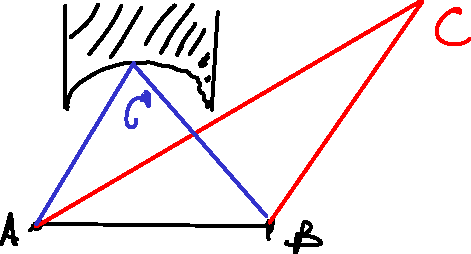
\includegraphics[width=0.5\linewidth]{max_S_with_restriction.pdf}
    \end{center}
    Любая конфигурация, кроме $C'$ улучшаема.
\end{example}

\begin{example}[Задача Томсона]
    Расположить $n$ единичных одноименных зарядов на $S^2$ с минимальной потенциальной энергией.
    \[E = \sum_{i \neq j} \frac{1}{\rho^2 (a_i, a_j)} \to \min\]
    Задача полностью не решена.
    Но мы знаем, что $\min$ достигается.
    $E: M \to \R$. $M \simeq S^2 \times S^2 \times ... \times S^2$ ($n$ раз).
    Но есть проблема с тем, что знаменатель может обратиться в 0.
    Исправим это:
    \[E'(a_1, a_2, ..., a_n) = \begin{cases}
            E(a_1, ..., a_n) & \rho(a_i, a_j) > \epsilon \\
            \displaystyle\sum_{\rho(a_i, a_j) > \epsilon} \frac{1}{\rho^2(a_i, a_j)} + \sum_{\rho(a_i, a_j) \le \epsilon} \frac{1}{\epsilon^2}
        \end{cases}\]
    $\epsilon$ взять такое, чтобы не мешало.
\end{example}

\begin{example}
    Есть $n$ сотрудников, существует $k$ групп из них, таких, что любые 2 группы пересекаются.
    Требуется доказать, что сотрудников можно расположить на окружности длиной 1,
    так чтобы любая группа была растянута по дуге не меньше чем $\frac{1}{3}$.

    Решение: пусть $x$ -- расстановка сотрудников, $S(x)$ -- минимальная длина дуги, которая покрывает какую-то группу.

    Хотим доказать: $\exists x_*: S(x_*) \ge \frac{1}{3}$.

    Возьмем $x_*$, для нее $S(x_*) = \max, S \ge \frac{1}{3}$
    \begin{center}
        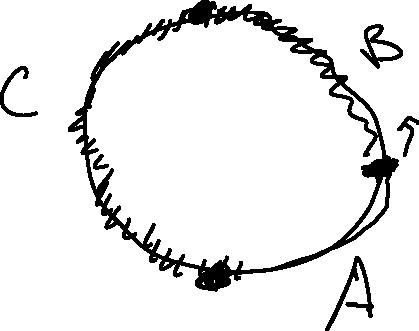
\includegraphics[width=0.5\linewidth]{staff_circle.pdf}
    \end{center}
\end{example}

\section{Локальная компактность}
\begin{definition}
    $X$ называется локально компактным, если
    \[\forall x_0\ \exists U_{x_0}: \Cl U_{x_0} \text{ компактна}\]
\end{definition}
\begin{theorem}[Компактификация по П.С. Александрову]
    $X$ -- локально компактное хаусдорфово пространство, тогда
    \[\exists \hat{X} = X \cup \{\infty\}\]
    $X$ -- подпространство $\hat{X}$ и $\hat{X}$ -- компактно и хаусдорфово.
\end{theorem}
\begin{example}
    \begin{gather*}
        \R \cup \{\infty\} \simeq S^1\\
        \R^2 \cup \{\infty\} \simeq S^2\\
        \R^n \cup \{\infty\} \simeq S^n
    \end{gather*}
\end{example}
\begin{proof}
    $\hat{X} = X \cup \{\infty\}$, но  какая топология?

    Пусть $U \subset \hat{X}$.
    Если $\infty \notin U$, то $U$ открыто в $\hat{X} \Leftrightarrow U$ открыто в $X$.

    Если $\infty \in U \implies U$ открыто $\Leftrightarrow X \setminus U$ компактно.

    Это топология: $X \setminus U$  компактно, значит по хаусдорфовости замкнуто.
    \begin{gather*}
        X \setminus \bigcup_{i \in I} U_i = \bigcap_{i \in I} (X \setminus U_i) \subset X \setminus U_{i_0}\\
        X \setminus \bigcap_{i = 1}^n U_i = \bigcup_{i = 1}^n (X \setminus U_i) \text{ -- компактно}
    \end{gather*}

    Это топология, $X \subset \hat{X}$ (в смысле топологии) (упражнение)

    Почему $\hat{X}$ компактен?

    $\{U_i\}_{i \in I}$ -- покрытие $\hat{X}$, $\infty \in U_{i_0}$.
    $X \setminus U_{i_0}$ -- компактно. (т.е. остальные множества покрывают компакт, можно выбрать конечное число)

    $\hat{X}$ -- хаусдорфово?

    $x,y \neq \infty$, тогда по хаусдорфовости $X\ \exists U_x, U_y: U_x \cap U_y = \varnothing$.

    $x, \infty$ как определить?
    $\exists U_x: \Cl U_x$ компактна. $U_\infty\coloneqq \hat{X} \setminus \Cl U_x$.
    $U_\infty$ открыто в $\hat{X}$.
\end{proof}
\begin{remark}
    Пересечение компактов не обязательно компакт!
    Но в хаусдорфовых пространствах пересечение компактов компакт.
    Потому что в хаусдорфовом пространстве компакт -- это замкнутое подмножество некоторого компакта.
\end{remark}
\begin{remark}
    Объединение конечного числа компактов -- компакт.
\end{remark}

\begin{example}
    $\hat{\Q} = \Q \cup \{\infty\}$.

    $\infty \in U$. $U$ открыто $\Leftrightarrow \Q \setminus U$ компактно.

    Докажем, что $\infty$ и $0$ не разделяются.
    Пусть они разделяются, тогда
    $U_0$ и  $U_\infty$, $U_0 \supset (-\epsilon, \epsilon) \cap \Q \implies \hat{\Q} \setminus U_\infty$ не компактно.
\end{example}

\begin{theorem}
    \

    \begin{enumerate}
        \item $X$ локально компактно и хаусдорфово, $x_0 \in X$, $U_{x_0}$ -- открытая окрестность $x_0$,
              тогда $\exists V_{x_0}: \Cl V_{x_0} \subset U_{x_0}$ и $\Cl V_{x_0}$ компактно.
              ($X$ локально компактно и хаусдорфово, $U \subset X$ открыто, тогда $U$ локально компактно и хаусдорфово)
        \item $X$ локально компактно и хаусдорфово, $K \subset X$ компакт.
              $K \subset G$, $G$ открытое, тогда $\exists$ открытое $G': G \supset \Cl G' \supset G' \supset K$
    \end{enumerate}
    \begin{center}
        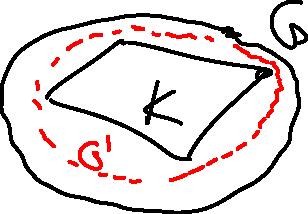
\includegraphics[width=0.3\linewidth]{local_compact_1.pdf}
    \end{center}
\end{theorem}
\begin{proof}
    \

    \begin{enumerate}
        \item $X$ локально компактно, значит существует $W_{x_0}: \Cl W_{x_0}$ компактно.
              $x_0 \in X\ \forall y \notin U$.
              Существуют непересекающиеся окрестности $W_{x_0,y}$ и $W_y$.
              Если $y \in \Cl W_{x_0} \cap (X \setminus U)$.
              $\Cl W_{x_0} \cap (X \setminus U)$ компакт (пересечение замкнутых -- замкнуто, оно подмножество $\Cl W_{x_0}$ -- компакт).

              $\{W_y\}$ -- покрытие $F \implies \exists$ конечное подпокрытие $y_1, ..., y_n: \{W_{y_i}\}_{i=1}^n$ -- подпокрытие $F$.

              $V_{x_0} = \bigcap_{i=1}^n W_{x_0,y_i}$ -- открытая окрестность $x_0$.
              \begin{gather*}
                  \Cl V_{x_0} \subset \bigcap_{i=1}^n \Cl W_{x_0, y_i} \subset U\\
                  \Cl W_{x_0, y_i} \subset X \setminus W_{y_i} \implies \bigcap \Cl W_{x_0, y_i} \subset X \setminus \left(\bigcup_{i=1}^n W_{y_i}\right) \subset U
              \end{gather*}
        \item $K \subset U, \forall x \in K \ \exists V_x: V_x \subset \Cl V_x \subset U$ (по 1 пункту).

              $\{V_x\}_{x \in K}$ -- покрытие $K$, значит существует конечное подпокрытие $\{V_{x_1}, ..., V_{x_k}\}$.
              \[G' \coloneqq \Cl \left(\bigcup_{i=1}^k V_{x+i}\right) \qedhere\]
    \end{enumerate}
\end{proof}

\end{document}